\chapter{\label{chap:spelunkbots}SpelunkBots}

\section{\label{section:game-ai-competitions}Competições de Inteligência
Artificial em Jogos Digitais}
Existe uma relação mutuamente benéfica entre a área de inteligência artificial e
jogos digitais.  De um lado, os jogos se beneficiam explorando conceitos,
técnicas e algoritmos de inteligência artificial com o intuito de enriquecer seu
conteúdo. O jogo \textbf{Black \&
White}\footnote{http://aigamedev.com/open/highlights/top-ai-games}, da
desenvolvedora \textit{Lionhead Studios}, por exemplo, incorporou as técnicas de
agentes BDI\footnote{\textit{Belief-Desire-Intention}, ou
Crença-Desejo-Intenção}, árvores de decisão e redes neurais para ditar o
comportamento de alguns dos personagens controlados pelo jogo.  Já o jogo
\textbf{F.E.A.R}, da desenvolvedora \textit{Monolith Productions}, utilizou os
conceitos de planejamento automático para aumentar o realismo das decisões
tomadas por seus agentes \cite{FEARPLANNING}.  Do outro lado, o campo da
inteligência artificial se beneficia ao utilizar os jogos como plataformas de
teste para suas técnicas e algoritmos. Jogos digitais são atraentes para
pesquisadores da área de inteligência artificial por uma série de fatores.
Primeiro, eles capturam a complexidade de situações do mundo real, são
relativamente simples e baratos de desenvolver, podem replicar inúmeras
situações e ambientes e até mesmo criar cenários impossíveis ou impraticáveis no
mundo real. Existem diversos gêneros de jogos, variando desde jogos educacionais
até jogos de tiro em primeira pessoa.  Segundo, jogos possuem a vantagem de
serem programas de computador, o que significa que, por muitas vezes, podem
acelerar a velocidade na qual testes são executados, ou ainda executar múltiplos
testes em paralelo. Finalmente, a natureza lúdica dos jogos são um ponto
importante a ser ressaltado, pois ajudam a motivar os pesquisadores, além de
resultar na adesão de novos pesquisadores.

Tendo este apanhado de informações em mente, pesquisadores e entusiastas da área
acabam desenvolvendo \textit{frameworks} de inteligência artificial em cima de
jogos existentes para servir de plataforma de teste. Um exemplo disso é o
\textbf{Brood War API}\footnote{bwapi.github.io}, um \textit{framework} para o
jogo \textit{StarCraft: Brood War}. Algumas vezes, contudo, são criados jogos
especificamente para pesquisa e experimentação, como foi o caso do projeto
\textbf{TORCS, The Open Racing Car
Simulator}\footnote{http://torcs.sourceforge.net/}, um simulador de corridas de
carro que permite que desenvolvedores programem a inteligência de carros e
compitam entre si.

Muitas vezes, os \textit{frameworks} de inteligência artificial desenvolvidos
abrem espaço para a criação de competições, servindo como base comum para o
desenvolvimento e aplicação de técnicas de inteligência artificial para os
concorrentes. Nestas disputas, os competidores são encorajados a resolver
problemas ou sub-problemas impostos pelo jogo em questão, sendo vencedores os
candidatos que melhor resolvê-los.

Geralmente, o problema proposto é o de jogar o jogo da maneira mais eficiente.
Existem pelo menos duas formas de se realizar uma avaliação objetiva dos
competidores. A primeira é através das métricas estipuladas pelo próprio jogo,
como alguma forma de pontuação ou tempo. A segunda é fazer com que os candidatos
joguem entre sí. Um exemplo disso é a competição que gira em torno de
\textbf{Vindinium}\footnote{vindinium.org}, um jogo para a plataforma
\textit{web}. Muitas vezes, os organizadores da competição optam por fazer uso
de um sistema de \textit{ranking}, expondo os resultados obtidos pelos
candidatos. A competição \textbf{The General Video Game AI
Competition}\footnote{gvgai.net}, que explora o problema de criar controladores
genéricos de jogos, utiliza este mecanismo.

Contudo, a proposta principal da disputa pode ser outra. A competição
\textbf{Mario AI Competition}, por exemplo, possuia como uma de suas metas a
criação de níveis interessantes para o jogo\footnote{marioai.org/home}. Já a
competição \textbf{2K Bot Prize} tinha como objetivo a criação de uma
inteligência artificial para o jogo \textit{Unreal Tournament 2004} que pudesse
enganar outros jogadores e fazê-los pensar que era um humano
jogando\footnote{http://www.aaai.org/Conferences/AIIDE/aiide.php}. Neste tipo
de torneio, a avaliação se dá de maneira subjetiva, visto que não existe uma
métrica numérica para determinar se um nível é interessante, por exemplo.

Os organizadores destas competições costumam, ao término da disputa,
disponibilizar os códigos-fonte de todos os candidatos. Assim, em versões
futuras da competição, os competidores terão a oportunidade de investigar quais
técnicas e algoritmos foram mais eficientes no passado. Os resultados das
competições costumam ser divulgados também em conferências como \textit{IEEE
Computational Intelligence and Games}\footnote{http://www.ieee-cig.org}
\textit{(CIG)} e \textit{AAAI Artificial Intelligence in Interactive Digital
Entertainment}\footnote{http://www.aaai.org/Conferences/AIIDE/aiide.php}
\textit{(AIIDE)}, além de conferências dedicadas a computação evolutiva,
\textit{game design}, aprendizado de máquina, entre outras.


%----------
\section{\label{section:spelunkbots}O \textit{SpelunkBots}}
Em 2014, Daniel Scales e Thomas Thompson, da Universidade de Derby no Reino
Unido, criaram o \textit{SpelunkBots}\cite{SPELUNKBOTSPAPER}, um
\textit{framework} que permite a programação de \textit{bots} para o jogo
Spelunky. Um dos objetivos dos criadores é utilizar a aplicação para criar uma
competição de inteligência artificial para o jogo. O \textit{framework} foi
desenvolvido utilizando uma combinação do código-fonte original do jogo
\textit{Spelunky} -- distribuído gratuitamente no \textit{website}
oficial\footnote{http://www.spelunkyworld.com/original.htm} --, o motor de
criação de jogos \textit{GameMaker} e uma solução \textit{DLL} (ou
\textit{Dynamic-link Library}) programada com a linguagem C++.


\subsection{\label{section:spelunkbots-usage}Modo de Uso}
Como o \textit{framework} possui acesso irrestrito ao código-fonte de
\textit{Spelunky}, a opção de programar a inteligência artificial utilizando a
linguagem de programação padrão do \textit{GameMaker}, a \textit{GML}, foi
incluida pelos criadores do programa. Contudo, esta opção não é adequada a
programadores mais experientes, visto que esta linguagem foi criada com o
intuito de fornecer a desenvolvedores de jogos iniciantes uma maneira fácil e
rápida de programar jogos e, justamente por este motivo, apresenta diversas
limitações de linguagem e não possui muitas bibliotecas auxiliares.  Além disso,
os arquivos \textit{.gml} só podem ser editados dentro do ambiente de
programação interno do \textit{GameMaker}.

Sabendo que o \textit{GameMaker} é capaz de executar código externo através de
\textit{DLLs}, os autores desenvolveram um projeto em C++ que gera uma solução
no formato \textit{DLL} para permitir que os usuários programem \textit{bots}
utilizando a linguagem de programação C++. Para programar em C++, portanto,  é
necessário usar uma ferramenta de compilação externa para gerar a solução
\textit{DLL}. O \textit{SpelunkBots} fornece um projeto em \textit{Visual Studio
2013} para auxiliar neste processo.

Assim, existem duas maneiras de se utilizar o \textit{SpelunkBots} para
programar uma inteligência artificial para \textit{Spelunky}: internamente,
através do \textit{GameMaker} e da \textit{GML}, ou externamente, através da
solução \textit{DLL} em C++. Desta maneira, o \textit{framework} fica acessível
tanto para programadores iniciantes quanto para programadores experientes.  A
Figura \ref{fig:spelunkbots-usage-diagram} ilustra a relação entre o
\textit{Spelunky}, o \textit{SpelunkBots} e as formas disponíveis de se realizar
a programação dos \textit{bots}.

\begin{figure}[htb!]
\centering
\begin{tikzpicture}[
    every node/.style={
        minimum width=4cm, minimum height=3em,
        text width=4cm,
        text centered,
        font=\small
    },
    box/.style={
        draw, rectangle,
        minimum width=5.3cm
    },
    inner box/.style={
        draw, rectangle
    }
]
    \matrix[row sep=1cm, column sep=1.5cm] {
        \node[rectangle] (spl) {Spelunky};                    &
                                                              &
        \\
        \node[inner box] (spb) {SpelunkBots};                 &
        \node[box]       (gml) {Código em GML};               &
        \\
        \node[box]       (dll) {Solução de DLLs do Spelunky}; &
        \node[box]       (c++) {Código em C++};
        \\
    };
    \node[draw, inner sep=.5cm, fit={(spl) (spb)}] {};

    \draw[->,>=latex] (gml.west) -- (spb.east);
    \draw[->,>=latex] (dll.north) -- (spb.south);
    \draw[->,>=latex] (c++.west) -- (dll.east);
\end{tikzpicture}
\caption {\label{fig:spelunkbots-usage-diagram}Diagrama exibindo a relação
entre o jogo Spelunky, a API SpelunkyBots e as linguagens de programação que
podem ser usadas para a interação com o jogo.}
\end{figure}


\subsection{Configurações da Ferramenta}
Antes de tentar executar o \textit{SpelunkBots}, é necessário entender como
realizar as configurações da ferramenta. As principais configurações que o
usuário deve modificar são a \textbf{escolha do \textit{bot}} a ser testado e o
\textbf{modo de execução} do jogo. Estas modificações são efetuadas dentro do
\textit{GameMaker} no projeto do \textit{framework}, chamado
\textit{spelunkbots.gmk}.

É possível que o usuário sinta a necessidade de desenvolver mais de uma
inteligência artificial ao mesmo tempo durante o uso da ferramenta.  Por
exemplo, pode desejar tentar solucionar diversos problemas específicos ou
realizar outros experimentos sem modificar o código-fonte do \textit{bot}
principal.  Para escolher o \textit{bot} que será executado, o usuário deve
modificar o arquivo de \textit{script} \textit{PlayerChoice} para escolher o
\textit{bot} que deseja testar.

Existem dois modos de execução em \textit{SpelunkBots}: o modo \textbf{TestMaps}
e o modo \textbf{Marathon}. No primeiro, a ferramenta executa o \textit{bot} em
uma série de mapas customizados, escolhidos pelo usuário. Este modo é perfeito
para testar as capacidades do \textit{bot} em cenários específicos ou difíceis
de encontrar durante uma partida comum. Já no segundo, executa o \textit{bot} em
uma série de mapas comuns, utilizando uma lista de sementes definidas pelo
usuário. Como as sementes são repassadas para o gerador de números
pseudo-aleatórios do algoritmo de geração de níveis, os \textit{layouts} dos
níveis serão sempre os mesmos. Este modo é ótimo para testar o \textit{bot} em
mapas normais do jogo, mas para ser bem sucedido, a inteligência artificial deve
estar muito preparada. Para escolher o modo de execução (e outros parâmetros
relacionados, como nome dos mapas, valores de sementes, número de execuções e
tempo limite por nível), o usuário deve modificar o arquivo de \textit{script}
\textit{LevelParameters}.


\subsection{Recebendo Informações do Jogo}
Uma das funcionalidades mais importantes da ferramenta é a disponibilização das
informações do jogo durante sua execução. As informações do jogo são divididas
em três grupos: \textbf{nodos}, \textbf{inimigos} e \textbf{objetos}:

\begin{description}
	\item[Nodos]
		O mapa do nível é dividido em nodos, e cada um destes nodos possui um
		tipo.  Para receber o tipo de um nodo em específico, a função da
		\textit{API} \textit{GetNodeState} deve ser chamada. Existe um total de
		1428 nodos em um mapa de \textit{Spelunky}.

	\item[Inimigos]
		Existem diversos tipos de inimigos em \textit{Spelunky}, e saber a
		localização deles é extremamente importante. Assim como as informações
		de nodo, cada inimigo possui um tipo associado a ele. Para determinar se
		um nodo possui um inimigo em específico, a função da \textit{API}
		\textit{GetIDOfEnemyInNode} deve ser usada.

	\item[Objetos]
		Em \textit{Spelunky}, existem diversos objetos com os quais o jogador
		pode interagir das mais diversas maneiras. Cada objeto possui um tipo
		associado a ele, para facilitar na distinção. Para determinar se um nodo
		possui um objeto em específico, a função da \textit{API}
		\textit{GetIDOfCollectableInNode} deve ser usada.
\end{description}

Além destas informações, o usuário pode receber dados sobre o estado do
\textit{bot}, como saber suas coordenadas, se ele está no ar, se movendo para a
direita ou esquerda, se ele está pendurado, entre outras. O apêndice
\ref{appendix:spelunkbots-variables} detalha os tipos de nodos, inimigos e
objetos e informações do estado do jogador.

Apesar de possibilitar ao desenvolvedor o resgate de informações sobre o jogo,
como o terreno, a posição de tesouros, armadilhas e inimigos, o objetivo do
\textit{framework} é fazer com que a informação recebida pelo \textit{bot} se
assemelhe ao máximo com a percepção de um jogador humano. Para tal, um sistema
de névoa de batalha (\textit{fog of war}) foi implementado, que serve para
limitar o conhecimento do ambiente que pode ser obtido pela inteligência
artificial.

Para objetos estáticos, uma vez que o jogador visualizou o objeto, ele poderá
receber informações sobre ele permanentemente. Um exemplo de objeto estático é o
terreno. Já para objetos dinâmicos, o \textit{bot} só receberá informações sobre
eles se estiverem sendo visualizados (dentro da tela do jogo) naquele momento.
Um exemplo de objeto dinâmico são os inimigos A Figura \ref{fig:spelunkbots-fow}
ilustra um exemplo de funcionamento do sistema, onde a área com o fundo nevoado
corresponde ao sistema de \textit{fog of war}.

\begin{figure}[htb!]
\centering
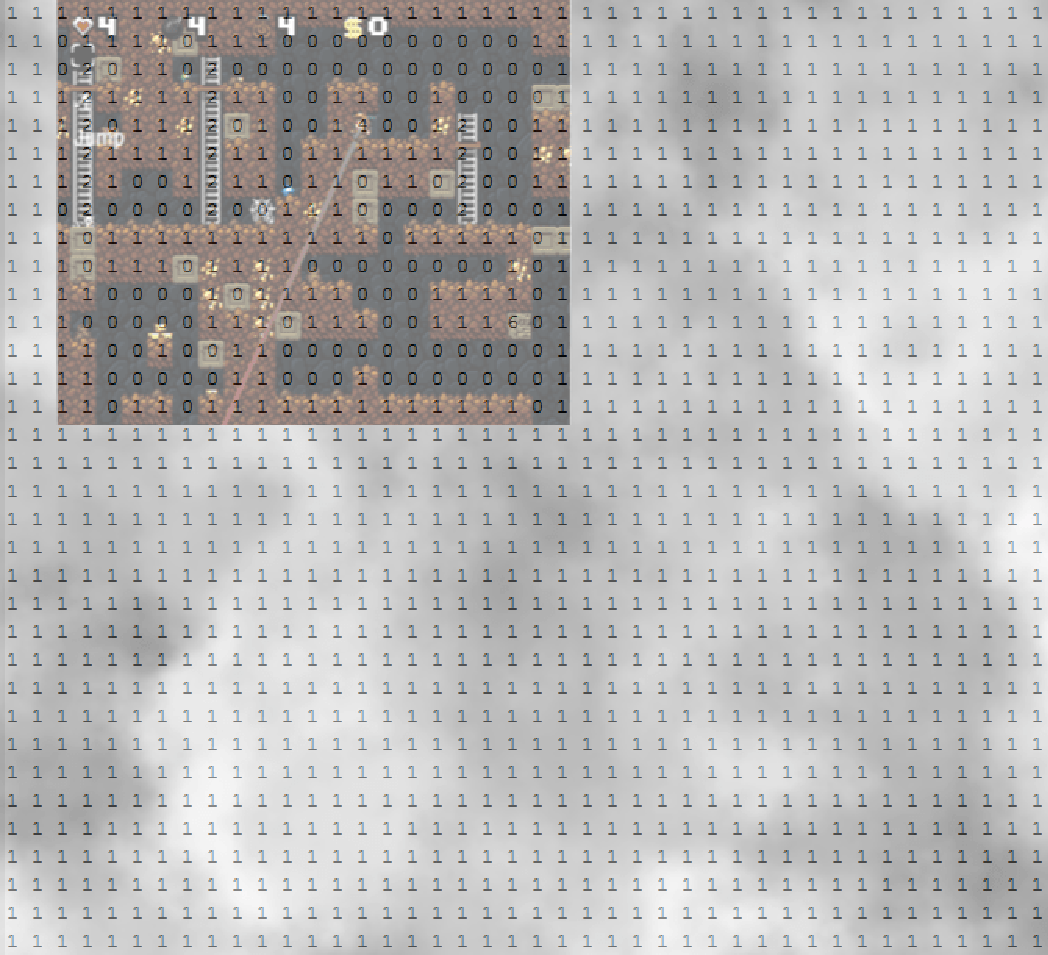
\includegraphics[width=.60\textwidth]{fig/spelunkbots-fow.pdf}
\caption {Visualização do sistema de \textit{fog of war} demonstrando a
diferença de informação recebida de nodos dentro e fora do campo de visão do
jogador.}
\label{fig:spelunkbots-fow}
\end{figure}

\todo[inline]{Dar crédito da foto (SpelunkBots)}

\subsection{Enviando Comandos para o \textit{Bot}}
Outra parte crucial da ferramenta é o envio de comandos para o \textit{bot}
durante a execução do jogo. Em \textit{SpelunkBots}, o envio de comandos é
controlado por uma série de variáveis \textit{booleanas} que estão mapeadas, uma
para uma, para os botões de controle (este mapeamento é apresentado no apêndice
\ref{appendix:spelunkbots-variables}). A cada etapa de execução, o usuário deve
modificar tais variáveis para \textit{verdadeiro} ou \textit{falso}, informando
para o \textit{framework} que comandos executar com o personagem.

O usuário não precisa se preocupar em reiniciar as variáveis de controle a cada
passo de execução, pois o programa já se encarrega disso: a cada fim de etapa de
execução, todas as variáveis são reiniciadas para o valor \textit{falso}. Ou
seja, se o usuário não enviar comandos em \textbf{todas as etapas de execução},
o \textit{bot} não se movimentará corretamente.
